\documentclass[a4paper,10pt,twoside,fleqn]{article}

% Note that if you want to use the \begin{equation} ... \end{equation}
% environment, you will have to include fleqn in the
% \documentclass[...]{...} options! 
% The top of your LaTeX file should then look like this:
% \documentclass[a4paper,10pt,twoside,fleqn]{article}
\usepackage[utf8]{inputenc}
\usepackage{clin}        % Stylefile for CLIN Journal
\usepackage{harvard}     % Bibliography Stylefile
%\usepackage{...,cgloss4e,avm,trees,tree-dvips,gb4e,ipa,graphicx}
                         % Whatever other packages you need
% Harvard:
% \cite{Covington}             (Covington 1994)
% \citeasnoun{Covington}       Covington (1994)
% \citeyear{Covington}         (1994)

\pagestyle{empty}

%%% own packages
\usepackage{booktabs}
\usepackage{chngcntr}
\usepackage{rotating}
\usepackage[section]{placeins}
\usepackage[super]{nth}

%%% commands
\newcommand{\overbar}[1]{\mkern 2.0mu\overline{\mkern-2.0mu#1\mkern-2.0mu}\mkern 2.0mu}


\begin{document}

\title{Towards Distinctive and Typical Style Features in Authorship}


\author{Carmen Klaussner$^*$ \email{klaussnc@tcd.ie}\\
{\normalsize \bf \c{C}a\u{g}ri \c{C}öltekin}$^{**}$ \email{c.coltekin@rug.nl}\\
{\normalsize \bf John Nerbonne}$^{**}$ \email{j.nerbonne@rug.nl}
\AND \addr{$^*$Trinity College Dublin, Ireland}
\AND \addr{$^{**}$University of Groningen, The Netherlands} }


\maketitle\thispagestyle{empty} % extra pagestyle command for first page

%To be filled in by the editors
%Please leave commented out
%\jmlrheading{vol}{year}{pages}{Submission date}{Publication date}{authors}
%\copyright

\begin{abstract}
Detection of stylistic elements in authorship studies is hampered
by the lack of a gold standard that would otherwise enable us to 
clearly evaluate our findings. In absence thereof, one generally 
resorts to choosing items for which an author shows a 
characteristic usage compared with other writers. 
In this line of work, we present both a measure for determining 
characteristic elements of an author that he uses consistently
over different works by examining different types of features, 
both lexical and syntactic ones.
For evaluation, we test the separation ability of the selected 
features by clustering the data set on their basis.

We apply both feature selection and evaluation in two different
studies of authorship. In the first, we compare Charles Dickens 
and Wilkie Collins, while the second one is contrasting the 
styles of Henry James and Mark Twain. Testing separation ability 
in clustering on highly representative and distinctive features 
returns results very close to the ideal clustering result.
\end{abstract}




\section{Introduction}
% this needs to include more references
The concept of \emph{style} in studies of authorship refers to the 
something like the feel of a piece of text, which might be less
tangible than style in other disciplines, such as art or music, 
where we use \emph{language} to express aspects of a 
painting or a piece of music, whereas for style in writing, 
we have to use the same tools that were used to create it. 

While traditional studies of authorship involve individual persona
judging upon what constitutes the style of an author, non-traditional
studies employ statistical techniques to discover the style of
an author. 
In either scenario, the development and investigation of suitable
methods of detection is hampered by the lack of a gold standard,
that would be able to indicate the method's closeness to 
returning true stylistic elements of an author. 
In absence thereof, the weight lies primarily on the method's 
theoretical appropriateness in the way it selects stylistic 
markers, which results in the need to understand our methods 
as well as their implications. 

\emph{Consistency} of stylistic markers has been somewhat of 
a central theme to studies of authorship, such as in early 
studies \cite{Mosteller2008}, which also emphasised collecting
larger number of markers to increase reliability of the result.
This has been continues in more recent studies as in 
the development of Burrow's Delta \cite{Burrows2002delta} 
and Zeta \cite{Burrows2007all} measures that build on
features representative for an author over a given number
of his texts, while distinguishing him from another/other 
author(s).

In this work, we consider \emph{Representativeness \& Distinctiveness}
\cite{prokic2012detecting}, a technique originating in dialectometry 
to select an author’s consistent features that are at the same time
also distinctive with respect to an opposing author’s sample.
Further, we propose a heuristic method for evaluation of those
selected features intended to measure how well they are able to
separate the data set into the correct groupings. 
As part of the analysis, we include both lexical and syntactic ones, 
such as simple word uni-grams, but also Part-of-Speech (POS) 
bi-grams/tri-grams.
The data consists of two separate authorship sets, where the first
consists of texts by two British authors, Charles Dickens and
Wilkie Collins and the second comprises writings by the two
American authors, Henry James and Mark Twain. 
%references of studies on those authors

Thus, in section~\ref{sec:data}, we describe the two data sets, while we 
introduce \emph{Representativeness \& Distinctiveness} 
in section~\ref{sec:method}. Further, section~\ref{sec:evaluation}
introduces and illustrates our proposed method of evaluation. 
Finally, in section~\ref{sec:experiments}, we describe our experiments
and results with respect to the two data sets and section~\ref{sec:conclusion}
closes the discussion. 


\section{The Data Sets} \label{sec:data}
For this study, we built two different author sets, one comparing Charles Dickens
and contemporary writer Wilkie Collins and the other one opposing Henry James 
to fellow American writer Mark Twain. 
All data was obtained from \emph{Project Gutenberg}\footnote{http://www.gutenberg.org/}
and the \emph{Internet Archive}\footnote{https://archive.org/}.

\subsection{Dickens vs. Collins}
% connection Dickens/Collins
Table~\ref{table:Dickens-data} and table~\ref{table:Collins-data} show Dickens'
and Collins' data set respectively, both comprising 27 documents.
Dickens' data set does not only contain documents by himself, but three books, namely, 
\emph{A Budget of Christmas Tales}, \emph{A House to Let} and \emph{No Thoroughfare}
are collaborations, where Dickens seems to have been main author.
In particular, the last two also include Wilkie Collins as author, where 
\emph{No Thoroughfare} was written by only Dickens and Collins. 
These were included, since they might be interesting with respect to stylistic properties.
If both authors persist in terms of style, these should be somewhat more difficult 
to classify than those written by only one of them.  
% exclude these from selection set 




% Dickens vs. Collins
\begin{table}[!ht]
%\caption{Dickens' data set.}
      \label{table:Dickens-data}
      \small
\begin{tabular}{c l l l} \\\hline \hline
\textbf{No.} 	& \textbf{Author} 	& \textbf{Texts} 			& \textbf{Abbr.} \\ \hline
1   		& Dickens 		& Bleak House 				& D1023     \\
2   		& Dickens		& Great Expectations			& D1400      \\
3		& Dickens      		& Little Dorrit     			& D963       \\
4		& Dickens      		& David Copperfield     		& D766        \\
5		& Dickens      		& A Christmas Carol     		& D19337       \\
6   		& Dickens		& Life And Adventures Of Martin Chuzzlewit	& D968        \\
7		& Dickens		& The Mystery of Edwin Drood		& D564   \\
8		& Dickens      		& A Tale of Two Cities                  & D98      \\
9		& Dickens		& Master Humphrey's Clock		& D588           \\
10		& Dickens		& The Battle of Life: A Love Story      & D40723              \\
11		& Dickens		& Life And Adventures Of Nicholas Nickleby	& D967          \\  
12		& Dickens		& Barnaby Rudge      			& D917             \\
13		& Dickens		& Sketches of Young Couples		& D916        \\
14		& Dickens		& The Uncommercial Traveller            & D914           \\
15		& Dickens		& Our Mutual Friend			& D883           \\
16		& Dickens		& Pictures From Italy			& D650    \\
17		& Dickens		& Sketches by Boz			& D882      \\
18		& Dickens		& A Child's History of England       	& D699  \\
19		& Dickens		& Reprinted Pieces			& D872   \\
20		& Dickens		& Dombey and Son			& D821     \\
21		& Dickens		& Oliver Twist				& D730        \\
22		& Dickens		&The Old Curiosity Shop			& D700         \\
23		& Dickens		& American Notes			& D675         \\
24		& Dickens		&The Pickwick Papers			& D580           \\
25		& Dickens    (et al.)   & A Budget of Christmas Tales		& Dal28198         \\
26		& Dickens (et al.)	& A House to Let			& Dal2324     \\
27		& Dickens (/Collins)     & No Thoroughfare			& DC1423       \\ \bottomrule
\end{tabular}
\end{table}


\begin{table}[!ht]
\caption{Collins' data set.}
\label{table:Collins-data}
\small
\begin{tabular}{c l l l } \\\hline \hline
\textbf{No.}	& \textbf{Author} 		& \textbf{Texts} 		& \textbf{Abbr.} \\ \hline
1		& Collins       		& After Dark			& C1626    \\
2		& Collins			& Antonina			& C3606        \\
3		& Collins			& Armadale			& C1895  \\
4		& Collins			& Man and Wife			& C1586      \\
5		& Collins			& Little Novels			& C1630    \\
6		& Collins			& Jezebel's Daughter		& C3633    \\
7		& Collins			& I Say No			& C1629       \\
8		& Collins			& Hide and Seek			& C7893  \\
9		& Collins			& Basil				& C4605 \\
10		& Collins			& A Rogue's Life		& C1588     \\
11		& Collins			& The Woman in White		& C583         \\
12		& Collins			& The Two Destinies		& C1624    \\
13		& Collins			& The Queen of Hearts		& C1917        \\
14		& Collins			& The New Magdalen		& C1623     \\
15		& Collins			& The Moonstone			& C155         \\
16		& Collins			& The Legacy of Cain		& C1975       \\
17		& Collins			& The Law and the Lady		& C1622         \\
18		& Collins			& The Haunted Hotel: A Mystery of Modern Venice	&    C170              \\
19		& Collins			& The Fallen Leaves		& C7894           \\
20		& Collins			& The Evil Genius		& C1627           \\
21		& Collins			& No Name			& C1438        \\
22		& Collins			& Poor Miss Finch		& C3632           \\
23		& Collins			& Rambles Beyond Railways	& C28367         \\
24		& Collins			& The Black Robe		& C1587      \\
25		& Collins			& Miss or Mrs.?			& C1621          \\
26		& Collins			& My Lady's Money		& C1628         \\
27		& Collins			& The Dead Alive		& C7891        \\
\bottomrule
\end{tabular}  
\end{table}


\subsection{James vs. Twain}
While Dickens and Collins seemed to have been close enough to collaborate on work,
this is a highly unlikely scenario for Henry James and Mark Twain. 
Although both being American writers close in age, they did not seemed to have
approved of each other as artists \cite{canby1951turn}. 
It is interesting to investigate to what extent this mutual dislike and 
disapprobation of each other 's work manifests itself in their writings
and what elements separate them. 
Table~\ref{table:Twain-data} and table~\ref{table:Twain-data} show 
James' and Twain's data sets, where James is represented with 25 and Twain
with 21 works. 


%James vs. Twain
\begin{table}[!htb]
    %\caption{Twain' and James' data set as part of the Twain vs. James' comparison.}
   % \label{table:TJ}
    \begin{minipage}{.62\linewidth}
    \centering
      \caption{Twain's data set.} %necessary???
      
      \label{table:Twain-data}
\begin{tabular}{c l l l} \\\hline \hline
\textbf{No.} 	& \textbf{Author} 	& \textbf{Texts} 			& \textbf{Abbr.} \\ \hline
1		&Twain			&Innocents Abroad			& T-ia\\ 
2		&Twain			&The Gilded Age: A Tale of Today	& T-tgaatot\\ 
3		&Twain			&Sketches New and Old			& T-snao\\
4		&Twain			&The Adventures of Tom Sawyer		& T-taots\\ 
5		&Twain			&A Tramp Abroad				& T-ata\\ 
6		&Twain			&Roughing It				& T-ri \\ 
7		&Twain			&The Prince and the Pauper		& T-tpatp\\ 
8		&Twain			&Life on the Mississippi		& T-lotm\\ 
9		&Twain			&The Adventures of Huckleberry Finn	& T-taohf\\ 
10		&Twain			&A Connecticut Yankee in King Arthur's Court& T-acyikac\\  
11		&Twain			&The American Claimant			& T-tac\\  
12		&Twain			&The Tragedy of Pudd'nhead Wilson	&T-ttopw\\   
13		&Twain			&Tom Sawyer Abroad			& T-tsa\\ 
14		&Twain			&Tom Sawyer Detective			& T-tsd\\ 
15		&Twain			&Personal Recollections of Joan Arc	& T-proja\\ 
16		&Twain			&Following the Equator: A Journey Around the World	&T-fteajatw\\
17		&Twain			&Those Extraordinary Twins 		&T-tet\\ 
18		&Twain			&A Double Barrelled Detective Story	& T-adbds\\ 
19		&Twain			&Christian Science			& T-cs\\
20		&Twain			&Chapters from My Autobiography		& T-cfma \\ 
21		&Twain			&The Mysterious Stranger		& T-tms\\ 
\bottomrule
\end{tabular}
\end{minipage}%
\vfill
    \begin{minipage}{.62\linewidth}
      \centering
      \caption{James' data set.} %necessary???
\label{table:James-data}
\begin{tabular}{c l l l } \\\hline \hline
\textbf{No.}	& \textbf{Author} 		& \textbf{Texts} 		& \textbf{Abbr.} \\ \hline
1		&James				&The American			&J-ta	\\
2		&James				&Watch and Ward			&J-waw	\\
3		&James				&The Europeans			&J-te	\\ 
4		&James				&Confidence 			&J-c	\\
5		&James				&Washington Square 		&J-ws	\\ 
6		&James				&Portrait of a Lady 		&J-poal	\\ 
7		&James				&Roderick Hudson		&J-rh	 \\
8		&James				&The Bostonians 		&J-tb	\\
9		&James				&Princess Casamassima 		&J-pc	\\
10		&James				&The Reverberator 		&J-tr	\\ 
11		&James				&The Aspern Papers		&J-tap	\\ %  novella
12		&James				&The Tragic Muse 		&J-ttm	\\ %
13		&James				&The Other House 		&J-toh	\\ %
14		&James				&What Maisie Knew        	&J-wmk	\\ 
15		&James				&The Spoils of Poynton  	&J-tsop	\\ %
16		&James				&Turn of the Screw		&J-tots	\\ %novella
17		&James				&The Awkward Age 		&J-taa	\\ %
18		&James				&The Sacred Fount		&J-tsf	\\ 
19		&James				&The Wings of the Dove		&J-twotd	\\  
20		&James				&The Golden Bowl 		&J-tgb	\\ %
21		&James				&The Ambassadors		&J-tamb	\\ 
22		&James				&The Outcry			&J-to	\\ %
23		&James				&The Ivory Tower (unfinished)	&J-tit	\\ %
24		&James				&The Sense of the Past (unfinished)&J-tsotp	\\%
25		&James				&In the Cage 			&J-itc	\\ % novella
\bottomrule
\end{tabular}

    \end{minipage} 
\end{table}



\section{Representativeness and Distinctiveness for Stylometry} \label{sec:method}
The statistical technique of Representativeness and Distinctiveness was 
originally conceived in the realm of dialectometry, where it has been
shown to detect lexical items able to distinguish different dialectical 
areas \cite{prokic2012detecting}.
This study dealt with dialect differences between different sites within 
a language area with respect to a choice of lexical items. 
The degree of difference between two sites is characterised by the aggregate 
differences of comparisons of all lexical items collected at 
each site. Thus, in the context of dialectrometry, 
\emph{Representativeness and Distinctiveness} is a measure to detect characteristic 
features (lexical items), that differ little within a group of sites 
and considerably more outside that group.
Characteristic features are chosen with respect to one group $g$ of sites 
$|g|$ within a larger group of interest $G$, where $|G|$ includes the sites 
$s$ both within and outside $g$.


In the context of stylometry, the method can be employed to detect elements for 
which an author is consistent throughout his own works while also separating him 
from others. Considering, for instance, a comparison between Dickens and fellow 
writer Collins on word features using a couple of novels of each writer, 
one first determines Dickens' representative terms, i.e. those words which he
uses consistently either frequently or infrequently over his works. 
In order to arrive at a combined measure, one then favours those representative 
terms of Dickens that Collins uses either inconsistently or consistently but with a
different frequency over his novels. The remaining group of words are considered 
to be Dickens' representative and distinctive terms when compared with Collins. 
% Since the analysis is directional, the degree of Representativeness of individual 
% features being different with respect to each author, comparisons are made twice
% - once from Dickens' to Collins' set and once from Collins' to Dickens' set. 
% This returns two individual author profiles, where features occurring in both 
% profiles are also consistent for both writers.
Thus, Representativeness and Distinctiveness bears similarities with both 
Burrow's Delta \cite{Burrows2002delta} and Zeta  \cite{Burrows2007all} in so far as
favouring consistent terms that are irregular in the opposing author's set. 
Additionally, it is also similar to Zeta in being dependent on the other set 
for the selection of distinctive terms out of the representative ones. 
Thus, formally the method of Representativeness and Distinctiveness is defined 
as follows: \\

\textsc{Representativeness} of a feature $f$ for document set $D$ is defined 
in eq.~\ref{eq.Rep}.


\begin{equation}\label{eq.Rep}
 \overbar{d_f^{D}} = \frac{2}{|D|^2 -|D|} \sum\limits_{d,d' \in D,d \neq d'} d_f(d,d')
\end{equation}



The \textsc{Distinctiveness} measure for comparing to outside documents corresponds 
to eq.~\ref{eq.Dis}.


\begin{equation}\label{eq.Dis}
 \overbar{d_f^{D'}} = \frac{1}{|D|(|DS| -|D|)} \sum\limits_{d \in D, d'\notin D} d_f(d,d')
\end{equation}


The distance $d_f$ between document $d$ and $d'$ with respect to feature $f$, is set as the 
absolute difference between the logarithm of the relative frequency of their respective
input values (eq.~\ref{eq.dist}).
The usual input are relative frequencies of the original term frequency weighting, which provide a 
better picture between the ratio of term frequency and document size. 
The logarithm lessens the effect of rather high frequencies. % this should be better

\begin{equation} \label{eq.dist}
 d_f(d,d') = |log(relFreq(f) - log(relFreq(f')|
\end{equation}


$\overbar{d_f^{D'}}$  and $\overbar{d_f^{D}}$ are standardized by using all 
distance values calculated for feature $f$ to yield the 
degree of representativeness and distinctiveness for
term $dt$ in $D$ with respect to $DS$ as defined in eq.~\ref{eq.comb}.
 
 \begin{equation}\label{eq.comb}
 dt = \frac{\overbar{d^{D'}_f} - \overbar{d_f} }{sd(d_f)} - \frac{\overbar{d^{D}_f} - \overbar{d_f}}{sd(d_f)}
\end{equation}


\paragraph{Comparing Authors on the basis of Representative Features}
% explain about different lists, how relevant for comparison 
% take intersection of Rep and dist. terms - yields true discriminatory terms for set for comparison - put emphasis on /extenuate differences 
% problem when take only one set, these terms will do nothing for similarity of other set among them 

In order to evaluate how well the chosen terms do separate the two authors, we motivate the choice of only selecting representative features from both author profiles. 
The issue in connection with using all discriminatory terms lies at the calculation of the $Distinctiveness$ measure. 
If we calculate representative and distinctive features for an author, we can be sure that the values for those 
terms are consistently similar for that author, while being different for the outside set. 
There are consequently two different scenarios with respect to a term \emph{being different} in the other author's set. 

1. The term $t_i$ is consistent in set $D$ with a high frequency. The same term $t_i$ is consistent in set the opposing author's set $nD$ with a low frequency. 
Thus, the term is representative and distinctive for both sets, even though we did not consider the $Representativeness$ for set $nD$. 
Obviously, the converse could also be true: a consistently low frequency for set $D$ and a consistently high frequency for the set $nD$.
This first case does not produce any issues for measuring similarity, since on the basis of these features there is is reliable similarity within sets and
accentuated differences between the sets. 

%% TOTD check references to DS because this is the whole set
%all the way trhough
2. The second possibility is the one that may cause problems. Assuming a representative and distinctive term for set $D$, with a frequency either high or low. 
However, the same term is not representative for set $nD$ and values may fluctuate from high to low. Although this term is not representative for $nD$, it
is distinctive from $D$ to $nD$, because it is constant in $D$ while not being so in $nD$. 
Clustering the dataset on the basis of these terms may create noise, since it will not show similarities for documents within $nD$ and 
may have occasional rather similar values to the ones in $D$ that rate it closer to documents in $D$.

\begin{figure}[!htb]
\minipage{0.3\textwidth}
\sf \textsc{Representativeness}
%\vspace{0.3cm}
  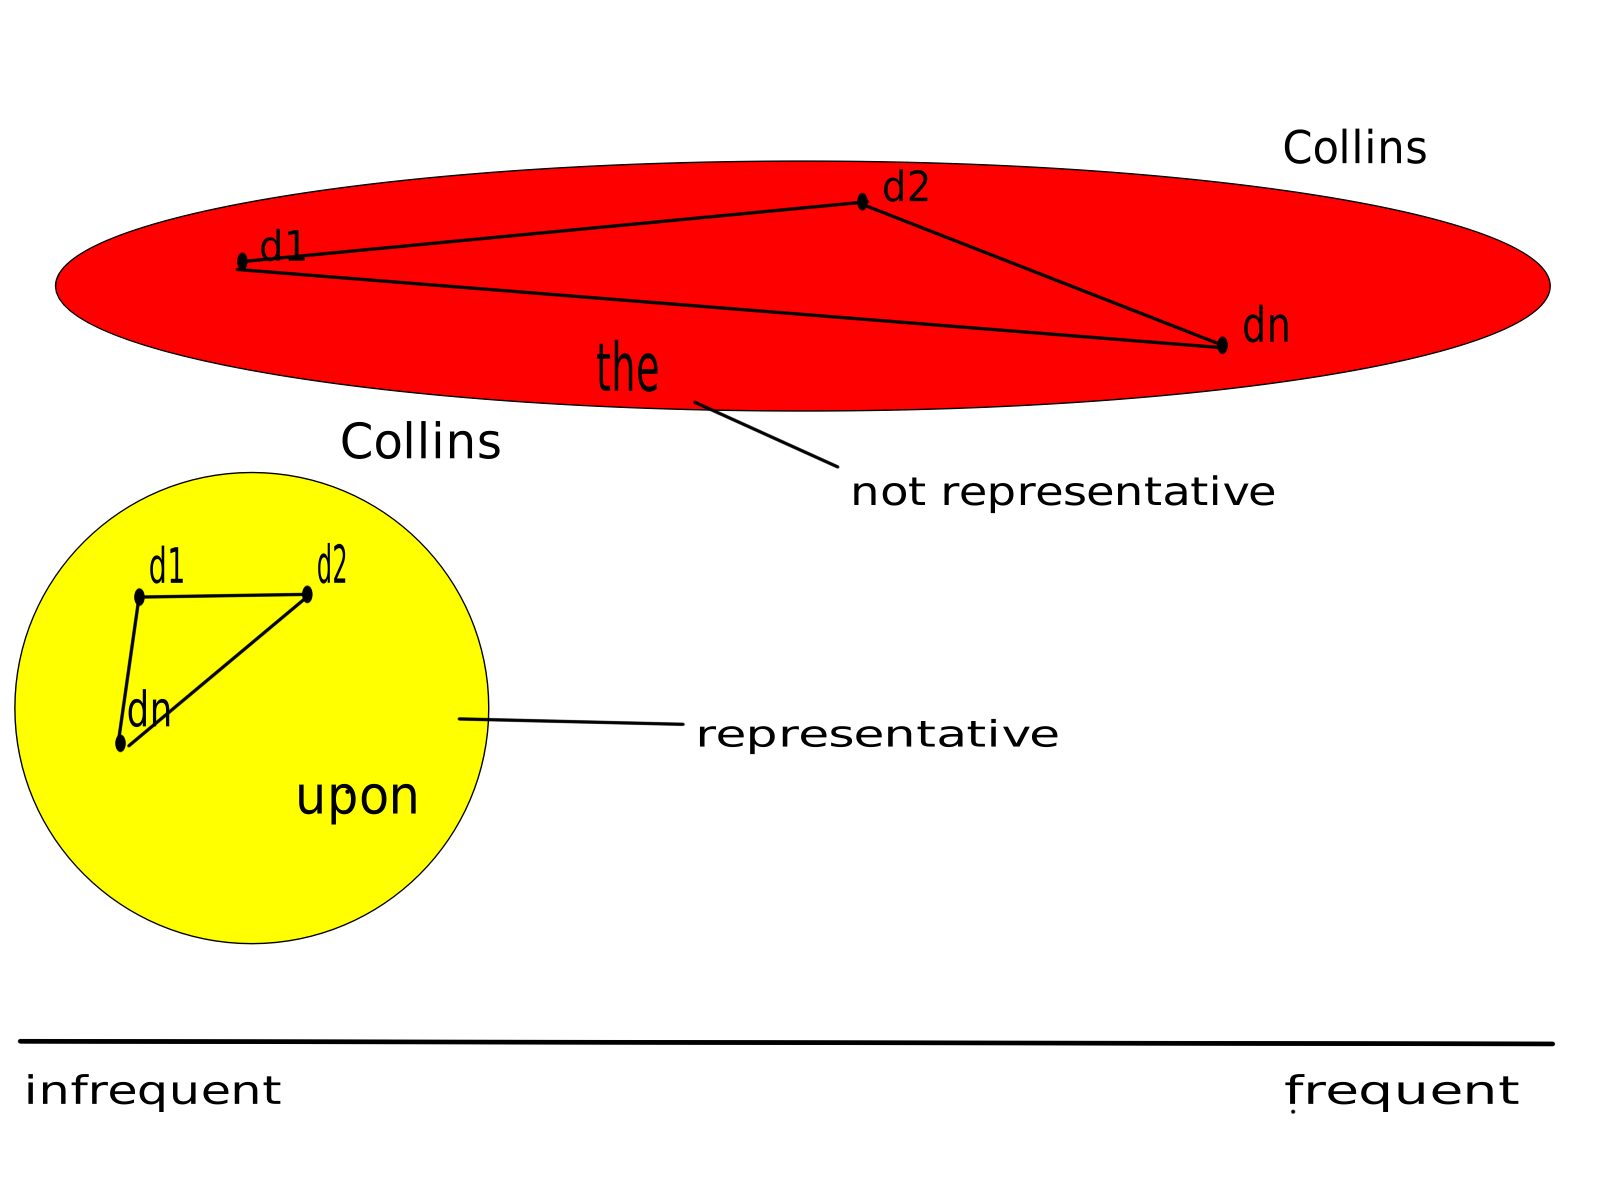
\includegraphics[scale=0.2,width=\linewidth]{figures/repres1-fin.png}
  \endminipage\hfill
\minipage{0.3\textwidth}
\sf \textsc{Distinctiveness} \\
{\scriptsize \textsc{Case 1}}\\
  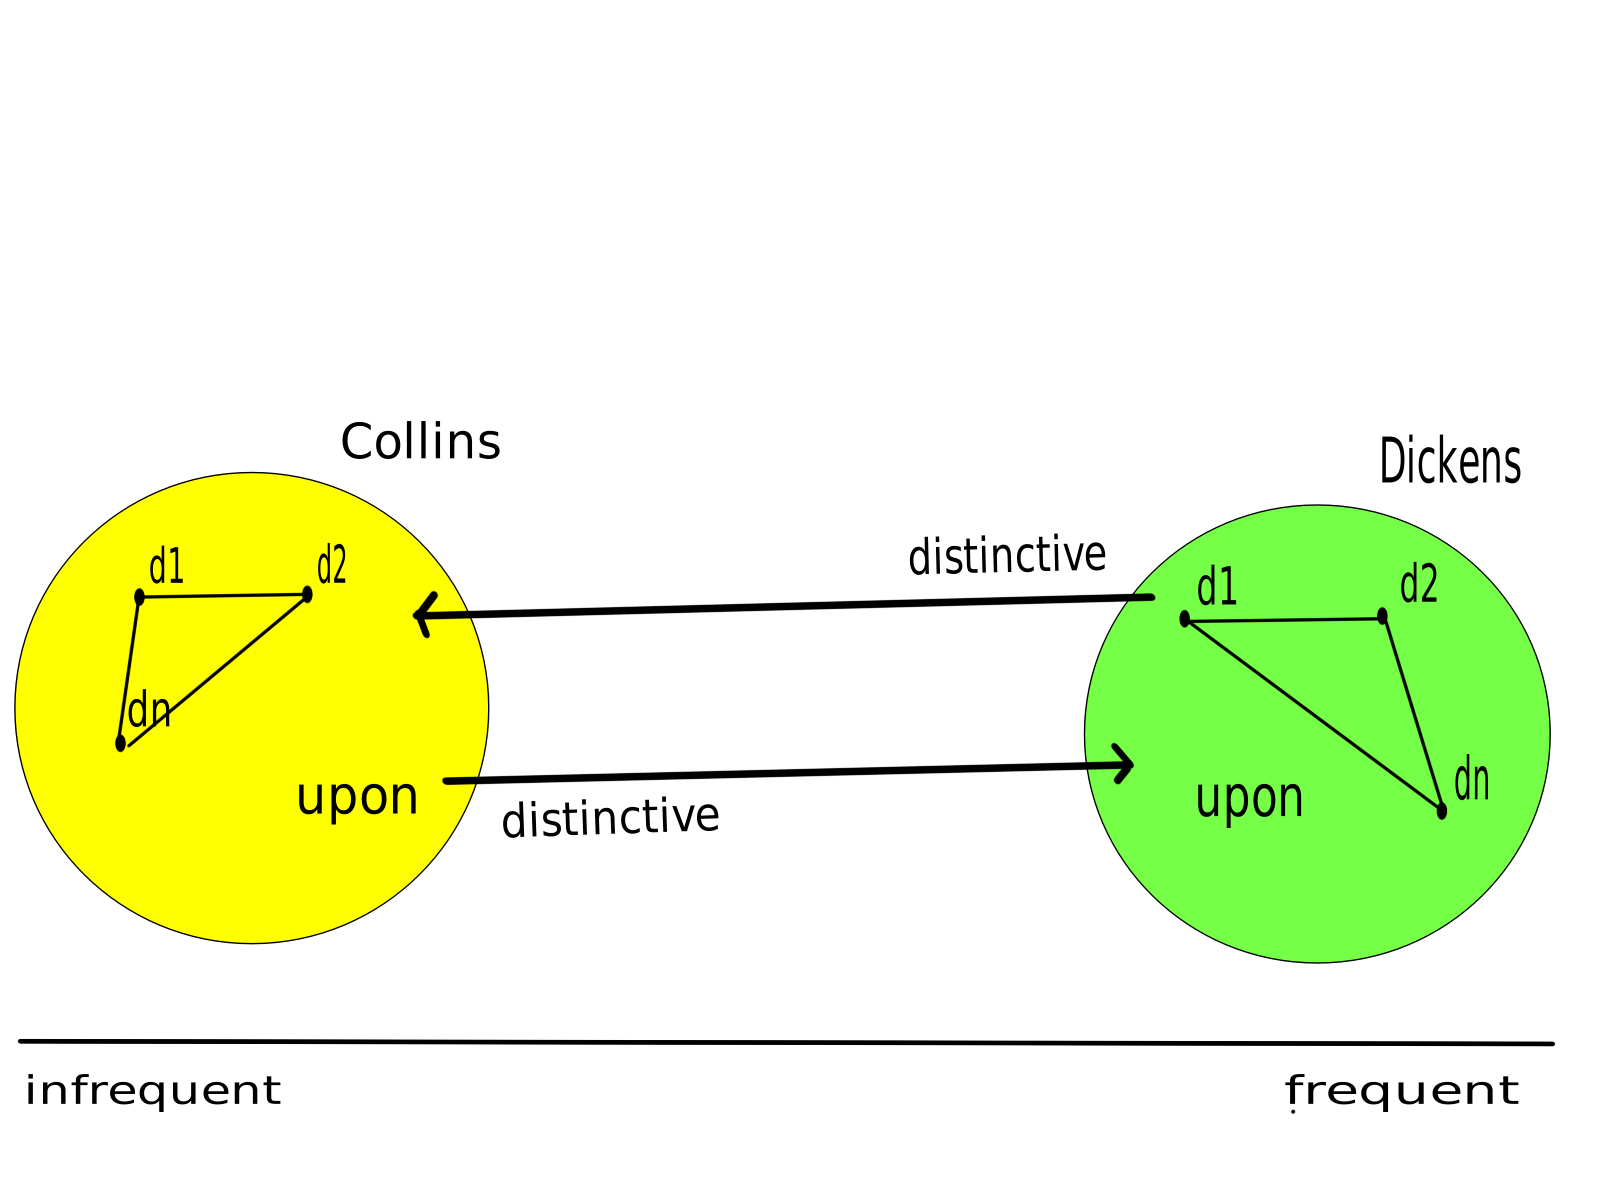
\includegraphics[scale=0.2,width=\linewidth]{figures/distinc1-fin.png}
\endminipage\hfill
\minipage{0.3\textwidth}%
\sf \textsc{Distinctiveness} \\
{\scriptsize \textsc{Case 2}}\\
  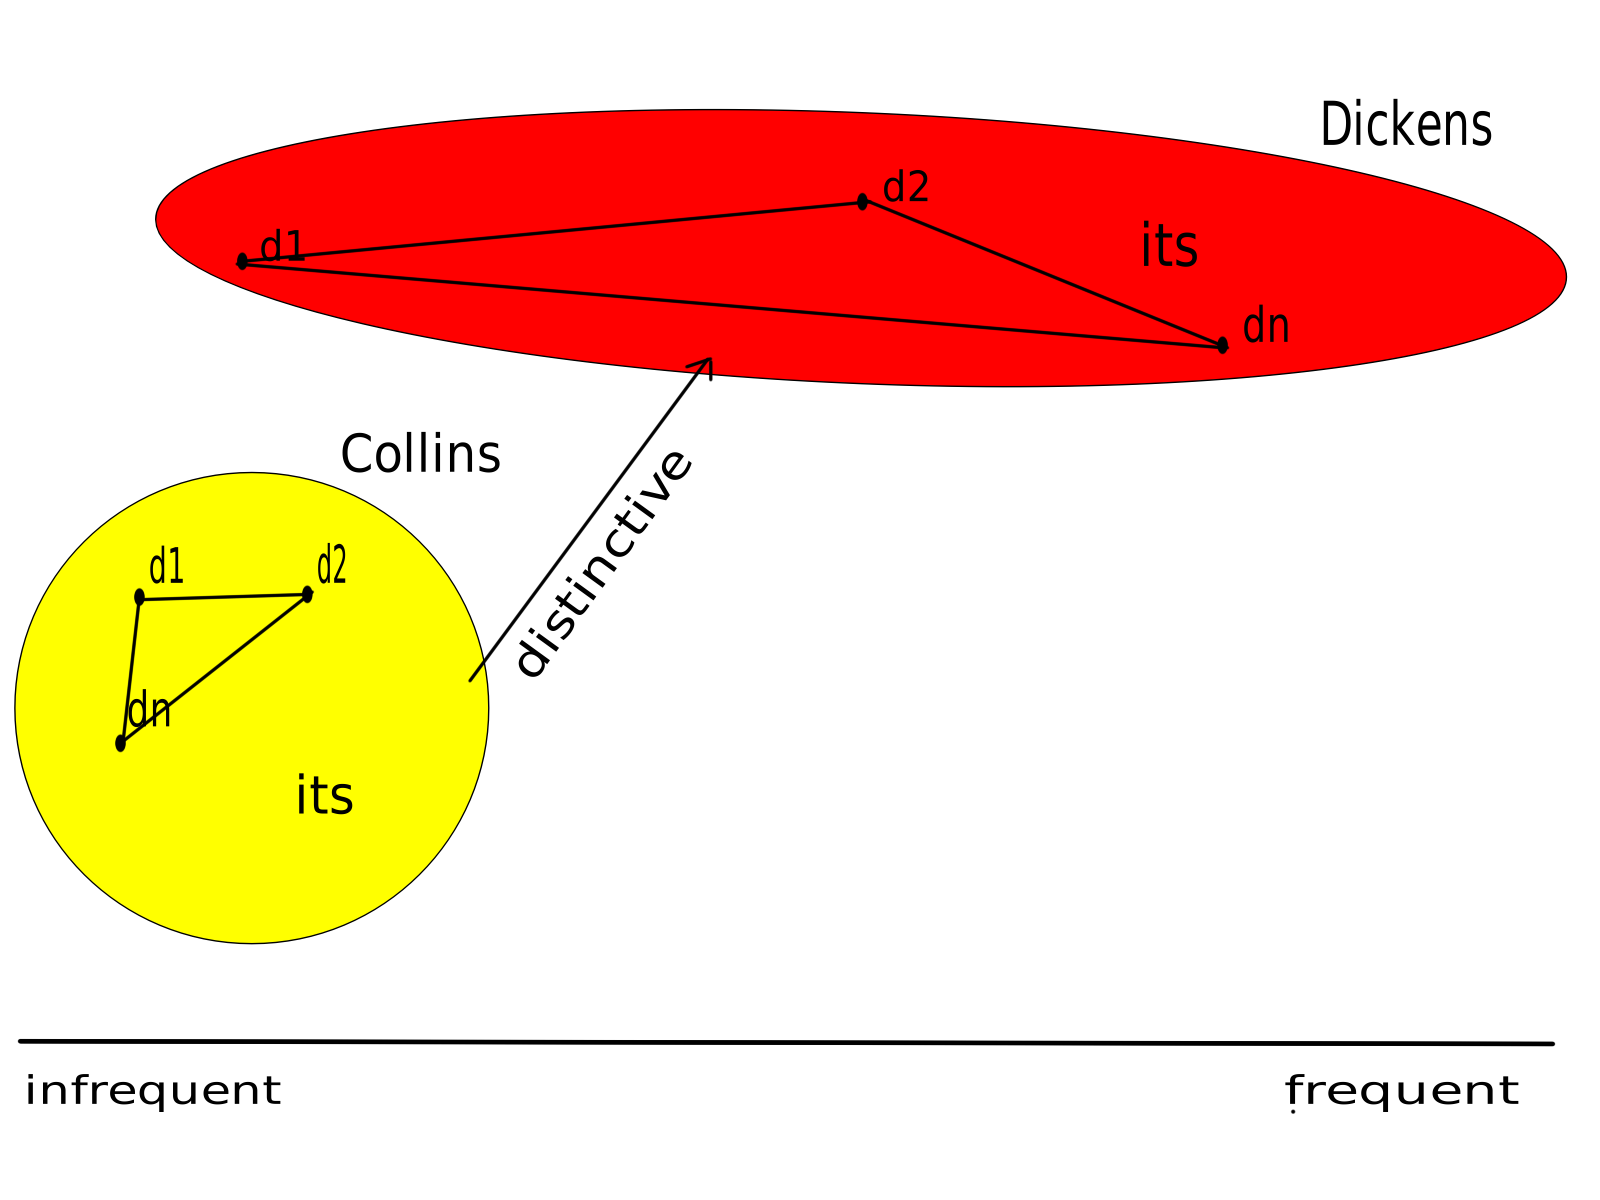
\includegraphics[scale=0.2,width=\linewidth]{figures/distinc2-fin.png}
 \endminipage
\end{figure}
 

\section{Evaluation through Clustering} \label{sec:evaluation}

Given a list of discriminatory terms for two different author sets, we would like to ascertain to what extent the collection of terms is able to 
highlight differences between the sets and identify distinct clusters grouping the documents of different authors. 
As has been shown before, the terms used for discrimination ability should be selected according to separation ability for both author sets. 
Ideally, frequencies with respect to all terms should be consistent and fairly complementary between two author sets, e.g.~Dickens uses \emph{upon} 
consistently and frequently and Collins uses the term consistently and infrequently. 
In order to test discrimination ability of a discriminatory term list for two authors, we build a dissimilarity matrix comparing all documents in 
the complete training set. 
%dividing by the number of terms in the $dt$ list, obtaining a mean distance for all document pairs given the discriminatory terms for that iteration. 
% The present solution emphasizes differences between the two sets, since we compare for the terms with
% the highest differences between the two sets. However, comparing within sets should not be problematic, since we consider
% terms both authors either employ frequently or avoid consistently, so within one author set, we expect values for either category to be closer, either low or high.

% \subsubsection{Dissimilarity Matrix} %quote? %http://www.statistics.com/index.php?page=glossary&term_id=512
% A dissimilarity matrix (or distance matrix) $D_M$ describes pairwise distances for $M$ objects, which results in a square symmetrical $M x M$ matrix, 
% where the $ij_{th}$ entry is equal to the value of a chosen measure of distinction $d$ between the $i_{th}$ and the $j_{th}$ object.
% The diagonal elements, comparing an object to itself are not considered or are usually equal to zero.
% A sample dissimilarity matrix is shown in matrix~\ref{ex:dissimMatrix}.
% Thus, in our case each document pair in $Dickens\cup nonDickens$ is compared based on the differences of $term_i$ in a given term list. 
% A common measure of distinction $d$ would be \emph{Manhattan} or \emph{Euclidean} distance.
% 
% 
% % \begin{equation}\label{ex:dissimMatrix}
% %  D_M = \begin{pmatrix} 0           & d_{12}         & \dots                                     & d_{1j}       \cr
% %                          d_{21} &   0           &       &        \vdots             \cr
% %                            \vdots                &                 &   \ddots      &   \vdots                   \cr
% %                          d_{j1}   &     \dots                           &        & 0                 \cr \end{pmatrix}
% % \end{equation}
% 
% Clustering on the basis of dissimilarity between objects, in this case documents can be done via hierarchical clustering.
% Agglomerative hierarchical clustering, for instance is an iterative clustering process, whereby cluster objects are joined together based on a distance measure between the 
% elements within the clusters. All elements begin in their own clusters and and are joined until the desired number of output clusters has been reached. 
% A common distance measure for joining clusters together is the \emph{complete link} method, which assesses closeness on the basis of the most distant elements 
% in two clusters $X$ and $Y$, in order to avoid the merging of two clusters based on only two single elements from each set being close.
% The distance $D(X,Y)$ between clusters $X$ and $Y$ is defined in eq.~\ref{eq:completeLink}, where $X$ and $Y$ are two sets of elements or clusters
% and $d(x,y)$ is the distance between elements $x \in X$ and $y \in Y$. 
% 
% 
% \begin{equation}\label{eq:completeLink}
%  D(X,Y)= \max_{x\in X, y\in Y} d(x,y) 
% \end{equation}
%  



\subsubsection{Adjusted Rand Index for Evaluation of Clustering} 
In addition to visual clustering that gives more of an intuition of separation between two sets, a clustering result can be evaluated by 
comparing two different partitions of a finite set of objects, namely the clustering obtained and the ideal clustering. 
For this purpose, we can employ the \emph{adjusted Rand Index} \cite{Hubert1985}, which is the corrected-for-chance version of the \emph{Rand Index}. 
Given a set $S$ of $n$ elements, and two clusterings of these points, $U$ and $V$, defined as   
$U = \{ U_1, U_2, \ldots , U_r \}$ and $V = \{ V_1, V_2, \ldots , V_s \}$ with $a_i$ and $b_i$ as the number of objects in cluster $U_i$ and $V_i$ respectively.
The overlap between U and V can be summarized in a contingency table~\ref{ex:continTable}. 
where each entry $n_{ij}$ denotes the number of objects in common between $U_i\; and\; V_j: n_{ij}=|U_i \cap V_j|$.

\begin{equation} \label{ex:continTable}
 \left[n_{ij}\right]= \bordermatrix{~
U\ V &	V_1 &  V_2 &	\ldots &	V_s 	&Sums \cr
U_1 &	n_{11} &	n_{12} &	\ldots 	&n_{1s} &	a_1 \cr
U_2 &	n_{21} &	n_{22} &	\ldots &	n_{2s} &	a_2\cr
\vdots &	\vdots &	\vdots &	\ddots &	\vdots &	\vdots\cr
U_r &	n_{r1} &	n_{r2} &	\ldots &	n_{rs} &	a_r\cr
Sums &	b_1 	&b_2 	&\ldots 	&b_s &    	\cr}
 \end{equation}
 
The adjusted form of the \emph{Rand Index} is defined in eq.~\ref{eq:ARI1} and more specifically given the contingency table~\ref{ex:continTable} 
in eq.~\ref{eq:ARI}, where $n_{ij}$, $a_i$, $b_j$ are values from the contingency table. 

\begin{equation}\label{eq:ARI1}
 AdjustedIndex = \frac{Index - ExpectedIndex}{MaxIndex - ExpectedIndex}
\end{equation}

% 
% \begin{equation}\label{eq:ARI}
%  ARI = \frac{ \sum_{ij} \binom{n_{ij}}{2} - [\sum_i \binom{a_i}{2} \sum_j \binom{b_j}{2}] / \binom{n}{2} }{ \frac{1}{2} 
%  [\sum_i \binom{a_i}{2} + \sum_j \binom{b_j}{2}] - [\sum_i \binom{a_i}{2} \sum_j \binom{b_j}{2}] / \binom{n}{2}}
% \end{equation}
% 
% 
% \begin{figure}[h!]
%  \caption{Dendrogram 'complete link' of dissimilarity Matrix on the basis of 300 input terms of Dickens and Collins.}
% \label{den:dissimM}
% \includegraphics[scale=0.6]{figure/dissimEx.pdf} %0.8200016
% \end{figure}

The index is bounded between [-1,1], with 0 being the expected value and 1 the highest positive correlation between two different clusterings. 
For illustration of using the two methods presented above, we consider an example of pairwise comparison of documents 
of a dataset of  $Dickens\cup Collins$, with 55 documents belonging to Dickens and 31 to Collins. 
This yields a 86 x 86 dissimilarity matrix containing all pairwise comparisons of documents in the set.  
Figure~\ref{den:dissimM} depicts an example dendrogram showing clustering based on a dissimilarity matrix with distances computed using the  \emph{complete link} measure. 
The \emph{adjusted Rand Index} corresponding to the clustering in figure~\ref{den:dissimM} is 0.82, so very close to the ideal separation, 
which is also confirmed, when we consider the small number of
misclassifications (3 for Dickens and 1 for Collins).  

 


\section{Experiments}\label{sec:experiments}



\section{Conclusion}\label{sec:conclusion}







%\nocite{Sag} % items in your bibliography file that are not cited in your text


\bibliographystyle{clin} 
\bibliography{biblio}  

%\appendix



% 
% \section*{Dickens vs. Collins}
% \begin{table}[h!] % Dickens 
% \caption{Dickens' data set as part of the Dickens vs. Collins comparison.}
% \label{table:Dickens-data}
% \scalebox{0.8}{
% \begin{tabular}{c l l l} \\\hline \hline
% \textbf{No.} 	& \textbf{Author} 	& \textbf{Texts} 			& \textbf{Abbr.} \\ \hline
% 1   		& Dickens 		& Bleak House 				& D1023     \\
% 2   		& Dickens		& Great Expectations			& D1400      \\
% 3		& Dickens      		& Little Dorrit     			& D963       \\
% 4		& Dickens      		& David Copperfield     		& D766        \\
% 5		& Dickens      		& A Christmas Carol     		& D19337       \\
% 6   		& Dickens		& Life And Adventures Of Martin Chuzzlewit	& D968        \\
% 7		& Dickens		& The Mystery of Edwin Drood		& D564   \\
% 8		& Dickens      		& A Tale of Two Cities                  & D98      \\
% 9		& Dickens		& Master Humphrey's Clock		& D588           \\
% 10		& Dickens		& The Battle of Life: A Love Story      & D40723              \\
% 11		& Dickens		&Life And Adventures Of Nicholas Nickleby	& D967          \\  
% 12		& Dickens		&Barnaby Rudge      			& D917             \\
% 13		& Dickens		& Sketches of Young Couples		& D916        \\
% 14		& Dickens		& The Uncommercial Traveller            & D914           \\
% 15		& Dickens		& Our Mutual Friend			& D883           \\
% 16		& Dickens		& Pictures From Italy			& D650    \\
% 17		& Dickens		& Sketches by Boz			& D882      \\
% 18		& Dickens		& A Child's History of England       	& D699  \\
% 19		& Dickens		& Reprinted Pieces			& D872   \\
% 20		& Dickens		& Dombey and Son			& D821     \\
% 21		& Dickens		& Oliver Twist				& D730        \\
% 22		& Dickens		&The Old Curiosity Shop			& D700         \\
% 23		& Dickens		& American Notes			& D675         \\
% 24		& Dickens		&The Pickwick Papers			& D580           \\
% 25		& Dickens     (et al.)  & A Budget of Christmas Tales		& Dal28198         \\
% 26		& Dickens (et al.)	& A House to Let			& Dal2324     \\
% 27		& Dickens (/Collins)     & No Thoroughfare			& DC1423       \\ \bottomrule
% \end{tabular}
% }
% \end{table}
% 
% \begin{table}[h!]% Collins 
% \caption{Collins' data set as part of the Dickens vs. Collins comparison.}
% \label{table:Collins-data}
% \scalebox{0.8}{
% \begin{tabular}{c l l l } \\\hline \hline
% \textbf{No.}	& \textbf{Author} 		& \textbf{Texts} 		& \textbf{Abbr.} \\ \hline
% 1		& Collins       		& After Dark			& C1626    \\
% 2		& Collins			& Antonina			& C3606        \\
% 3		& Collins			& Armadale			& C1895  \\
% 4		& Collins			& Man and Wife			& C1586      \\
% 5		& Collins			& Little Novels			& C1630    \\
% 6		& Collins			& Jezebel's Daughter		& C3633    \\
% 7		& Collins			& I Say No			& C1629       \\
% 8		& Collins			& Hide and Seek			& C7893  \\
% 9		& Collins			& Basil				& C4605 \\
% 10		& Collins			& A Rogue's Life		& C1588     \\
% 11		& Collins			& The Woman in White		& C583         \\
% 12		& Collins			& The Two Destinies		& C1624    \\
% 13		& Collins			& The Queen of Hearts		& C1917        \\
% 14		& Collins			& The New Magdalen		& C1623     \\
% 15		& Collins			& The Moonstone			& C155         \\
% 16		& Collins			& The Legacy of Cain		& C1975       \\
% 17		& Collins			& The Law and the Lady		& C1622         \\
% 18		& Collins			& The Haunted Hotel: A Mystery of Modern Venice	&    C170              \\
% 19		& Collins			& The Fallen Leaves		& C7894           \\
% 20		& Collins			& The Evil Genius		& C1627           \\
% 21		& Collins			& No Name			& C1438        \\
% 22		& Collins			& Poor Miss Finch		& C3632           \\
% 23		& Collins			& Rambles Beyond Railways	& C28367         \\
% 24		& Collins			& The Black Robe		& C1587      \\
% 25		& Collins			& Miss or Mrs.?			& C1621          \\
% 26		& Collins			& My Lady's Money		& C1628         \\
% 27		& Collins			& The Dead Alive		& C7891        \\
% \bottomrule
% \end{tabular}
% }
%  \end{table}
% 



\end{document}
